\section{Theorie}
\label{sec:Theorie}
\subsection{Kapazitiv gekoppelte Schwingkreise}
Zwei elektrische Schwingkreise, die jeweils aus einer Kapazität C und einer
Induktivität L bestehen, sind über einen Kopplungskondensator $C_k$ gekoppelt.
Der schematische Aufbau eines solchen gekoppelten Schwingkreises ist in Abbildung
\ref{fig:schwingkreis} zu sehen.
\begin{figure}
  \centering
  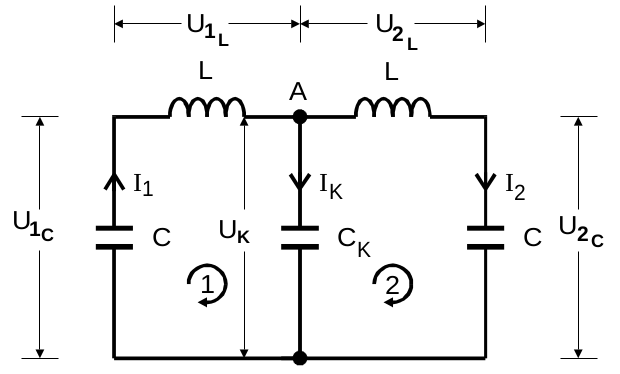
\includegraphics[width=0.8\textwidth]{schwingkreis.png}
  \caption{Aufbau zweier Schwingkreise, die mit einem Kopplungskondensator
  gekoppelt sind \cite{sample}.}
  \label{fig:schwingkreis}
\end{figure}
Mit den Kirchhoffschen Gesetzen kann man die Zeitabhänigkeit der Ströme $I_1$
und $I_2$ berechnen.
Aus der Knotenregel folgt
\begin{equation}
  I_\text{K} = I_1 - I_2 ,
  \label{eqn:knoten}
\end{equation}
und mit der Maschenregel folgt für die erste und die zweite Masche
\begin{align}
  U_{1_\text{C}} + U_{1_\text{L}} + U_\text{K} &= 0
  & U_{2_\text{C}} + U_{2_\text{L}} + U_\text{K} &= 0 .
  \label{eqn:maschen}
\end{align}
Für die Kondensatorspannung gilt dabei $U_\text{C} = \frac{1}{C}\int I \symup{d}t$
und für die Spulenspannung $U_\text{L} = L \dot{I}$.
Diese Beziehungen führen mit einmaliger Ableitung nach der Zeit auf folgendes
gekoppeltes Differentialgleichungssystem:
\begin{equation}
  L \ddot{I_1} + \frac{1}{C} I_1 + \frac{1}{C_\text{K}} (I_1 - I_2) = 0
  \label{eqn:gekoppelte_dgl_1}
\end{equation}
\begin{equation}
  L \ddot{I_2} + \frac{1}{C} I_2 + \frac{1}{C_\text{K}} (I_1 - I_2) = 0.
  \label{eqn:gekoppelte_dgl_2}
\end{equation}
Durch Einführung neuer Variablen $\alpha = (I_1 + I_2)$, also der Summe der
Einzelströme, und $\beta = (I_1 - I_2)$, also der Differenz der Einzelströme
können die Differentialgleichungen entkoppelt werden:
Aus Gleichung \eqref{eqn:gekoppelte_dgl_1} + \eqref{eqn:gekoppelte_dgl_2} erhält
man
\begin{equation}
  \ddot{\alpha} + \frac{1}{L C} \alpha = 0
  \label{eqn:dgl1}
\end{equation}
und aus \eqref{eqn:gekoppelte_dgl_1} - \eqref{eqn:gekoppelte_dgl_2}
\begin{equation}
  \ddot{\beta} + \left(\frac{1}{L C} + \frac{2}{L C_\text{K}}\right) \beta = 0.
  \label{eqn:dgl2}
\end{equation}
Nun kann man leicht erkennen, dass dies zwei lineare homogene Differentialgleichungen
wie die eines harmonischen Oszillators sind. Man erhält mit dem Lösungsansatz
$x(t) = x_0 cos (\omega t)$ und $\omega_1 = \sqrt{\frac{1}{LC}}$ sowie
$\omega_2 = \sqrt{\frac{1}{L}\left(\frac{1}{C}+\frac{2}{C_\text{K}}\right)}$ leicht die
Lösungen
\begin{equation}
  \alpha(t) = \alpha_0 \cos\left(\frac{1}{\sqrt{L C}}t\right)
  \label{eqn:alpha}
\end{equation}
mit $\alpha_0 = (I_{1,0} + I_{2,0})$, also der Summe der Ströme zum Zeitpunkt
$t = 0$, sowie
\begin{equation}
  \beta(t) = \beta_0 \cos\left(\sqrt{\frac{1}{L}\left(\frac{1}{C}+
  \frac{2}{C_\text{K}}\right)}\right)
\end{equation}
mit $\beta_0 = (I_{1,0} - I_{2,0})$, also der Differenz der Ströme zum Zeitpunkt
$t = 0$.
Aus der Beziehung $\omega = 2 \pi \nu$ folgen die Schwingungsfrequenzen
\begin{equation}
  \nu^{+} = \frac{1}{2 \pi \sqrt{L C}}
  \label{eqn:frequenz_puls}
\end{equation}
und
\begin{equation}
  \nu^{-} = \frac{\sqrt{\frac{1}{L}\left(\frac{1}{C}+\frac{2}{C_\text{K}}\right)}}{2 \pi}.
  \label{eqn:frequenz_minus}
\end{equation}

Werden $\alpha$ und $\beta$ nun resubstituiert, so erhält man die folgenden Lösungen
für $I_1(t)$ und $I_2(t)$:
\begin{equation}
  I_1(t) = \frac{1}{2} (I_{1,0} + I_{2,0}) \cos(2\pi\nu^{+}t)
  + \frac{1}{2} (I_{1,0} - I_{2,0}) \cos(2\pi\nu^{-}t)
  \label{eqn:I1}
\end{equation}
\begin{equation}
  I_2(t) = \frac{1}{2} (I_{1,0} + I_{2,0}) \cos(2\pi\nu^{+}t)
  - \frac{1}{2} (I_{1,0} - I_{2,0}) \cos(2\pi\nu^{-}t).
  \label{eqn:I2}
\end{equation}
Wichtige Spezialfälle des gekoppelten Systems sind die Fundamentalschwingungen.

Starten beide Schwingkreise mit der gleichen Amplitude, also $I_{1,0} = I_{2,0}$,
und sind zudem noch in Phase ($\Delta \Phi = 0$), so hängt die Schwingung nur noch
von der Summenschwingung und nicht mehr von der Differenzenschwingung ab. Dies
hat zur Folge, dass das gesamte System ständig in Phase ist und mit der Frequenz
$\nu^{+}$ schwingt. Am Koppelkondensator liegt dabei keine Spannung an.

Wenn das System stattdessen mit einer Phasenverschiebung von $\Delta \Phi = \pi$
und gleicher Amplitude startet (also $I_{1,0} = - I_{2,0}$), schwingt das System
mit der Frequenz $\nu^{-}$, welche vom Koppelkondensator abhängig ist und größer
als $\nu^{+}$.

Ein dritter wichtiger Fall ist die Schwebung. Diese tritt auf, wenn zu Beginn
nur einer der Schwingkreise eine Amplitude ungleich Null ($I_{1,0} \neq 0$)
besitzt, während der andere Schwingkreis ruht ($I_{2,0} = 0$). Die Gleichungen
für die Ströme $I_1(t)$ und $I_2(t)$ lassen sich mit Hilfe von Additionstheoremen
für Cosinus und Sinus zu
\begin{equation}
  I_1(t) = I_{1,0} \cos\left(\frac{1}{2}(\omega^{+}+\omega^{-})t\right)
  \cos\left(\frac{1}{2}(\omega^{+}-\omega^{-})t\right)
  \label{eqn:schwebung_I1}
\end{equation}
und
\begin{equation}
  I_1(t) = I_{1,0} \sin\left(\frac{1}{2}(\omega^{+}+\omega^{-})t\right)
  \sin\left(\frac{1}{2}(\omega^{+}-\omega^{-})t\right)
  \label{eqn:schwebung_I2}
\end{equation}
umformen.
Wählt man $\nu^{+} \approx \nu^{-}$, also $C_\text{K} \gg C$, dann schwingt die
Systeme mit der Frequenz $\frac{1}{2}(\nu^{+} + \nu^{-})$. Die Amplitude ändert
sich dabei mit der Schwebungsfrequenz $\nu^{-} - \nu^{+}$. Der graphische Verlauf
der zeitlichen Änderung der Schwingungsamplituden ist in Abbildung \ref{fig:schwebung}
zu sehen.
\begin{figure}
  \centering
  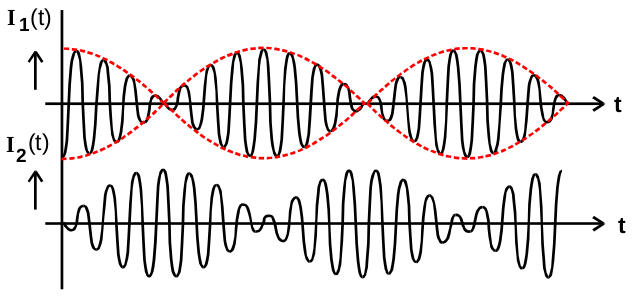
\includegraphics[width=\textwidth]{schwebung.png}
  \caption{Zeitlicher Verlauf der Stromamplituden bei Schwebung \cite{sample}.}
  \label{fig:schwebung}
\end{figure}
Die Energie pendelt periodisch zwischen den zwei Schwingkreisen hin und her.

\subsection{Frequenzabhänigkeit des Stromes im gekoppelten Schwingkreis}
Im Folgenden wird ein gekoppelter Schwingkreis von außen mit einer Sinusschwingung
angeregt, so dass dieser eine erzwungene Schwingung ausführt. Alle verlustbehafteten
Vorgänge werden dabei durch je einen ohmschen Widerstand pro Schwingkreis
dargestellt. Der Aufbau eines solchen Schwingkreises ist in Abbildung
\ref{fig:erzwungene_schwingung} zu sehen.
\begin{figure}
  \centering
  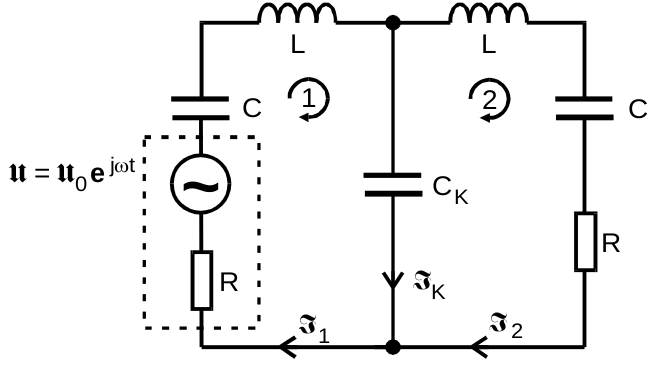
\includegraphics[width=0.9\textwidth]{erzwungene_schwingung.png}
  \caption{Aufbau eines verlustbehafteten gekoppelten Schwingkreises mit erzwungener
  Schwingung \cite{sample}.}
  \label{fig:erzwungene_schwingung}
\end{figure}

\noindent Mit der Maschenregel werden die Beziehungen
\begin{align*}
  (Z_\text{C} + Z_\text{L} + Z_{C_\text{K}} + Z_\text{R})I_1 - Z_{C_\text{K}} I_2 &= U \\
  (Z_\text{C} + Z_\text{L} + Z_{C_\text{K}} + Z_\text{R})I_2 - Z_{C_\text{K}} I_1 &= 0
\end{align*}
mit den Impedanzen $Z_\text{C} = \frac{-i}{\omega C}$, $Z_\text{L} = i\omega L$
und $Z_\text{C} = R$ aufgestellt. Es wird die Abkürzung
\begin{equation}
  Z(\omega) = \omega L - \frac{1}{\omega}\left(\frac{1}{C}+\frac{1}{C_\text{K}}\right)
  \label{eqn:z_omega}
\end{equation}
eingeführt. Für den Betrag von $I_2$ erhält man dann mit dem Leitwert $|\symfrak{L}|$
\begin{equation}
  \left|I_2\right| = |U| \frac{1}{\sqrt{4\omega^2 C_\text{K}^2 R^2 Z(\omega)^2
  + \left(\frac{1}{\omega C_\text{K}} - \omega C_\text{K} Z(\omega)^2
  + \omega R^2 C_\text{K}\right)^2}} = |U|\cdot|\symfrak{L}|.
  \label{eqn:betrag_I2}
\end{equation}
Für $\omega \to 0$ und $\omega \to \infty$ geht $|I_2|$ gegen Null. Bei den
Fundamentalfrequenzen $\omega^{+}$ und $\omega^{-}$ werden die Maxima der Leitwerte
erreicht, welche mit
\begin{equation}
  |\symfrak{L}(\omega^{+})| \approx |\symfrak{L}(\omega^{-})| \approx \frac{1}{2R}
  \label{eqn:naeherung_maxima}
\end{equation}
genähert werden können.



\cite{sample}
